\chapter{Preface}

This thesis was prepared at DTU Compute in fulfilment of the requirements for acquiring an M.Sc. in Engineering.

This thesis focus on non-conditional and conditional action schema learning.
It extends the work of \cite{Walsh2008}, but also uses ideas from the scientific method which has evolved through many greek philosophers, and we have been heavily inspired by the works of \cite{popper1959a}.

This thesis will provide a proposal about a general agent learning algorithm, a complete a analysis of non-conditional action learning; and a framework and framing of the problems with conditional action learning, and provide initial proposals a solution.
%==================================================================================================
% SIGNATURE AREA
%==================================================================================================
\vspace{20mm}
\begin{center}
    \hspace{20mm} Lyngby, \thesishandin-\thesisyear
    \vspace{5mm}
    \newline
  %Update signature image file in line below
    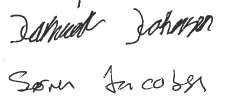
\includegraphics[scale=0.8]{Graphics/signatures}
\end{center}
\begin{flushright}
    \thesisauthor
\end{flushright}
% % % EOF % % %
